\documentclass[11pt]{article}
\usepackage[textwidth=18.0cm, textheight=23.0cm, top=2.0cm]{geometry}
\usepackage{pst-all}
\usepackage{amssymb}
\usepackage{tikz}
\usepackage{underscore}\begin{document}
\pagestyle{empty}


ClassName: \underline{\textbf{Class_02.2bp-1}}
\par
BinSize: \underline{\textbf{30 × 30}}
\par
ReduceSize: \underline{\textbf{30 × 30}}
\par
TypeNum: \underline{\textbf{18}}
\par
Num: \underline{\textbf{20}}
\par
OutS: \underline{\textbf{900}}
\par
InS: \underline{\textbf{433}}
\par
Rate: \underline{\textbf{0.481}}
\par
UB: \underline{\textbf{1}}
\par
LB0: \underline{\textbf{1}}
\par
LB: \underline{\textbf{1}}
\par
LBWithCut: \underline{\textbf{1}}
\par
NodeCut: \underline{\textbf{0}}
\par
ExtendedNodeCnt: \underline{\textbf{1}}
\par
GenNodeCnt: \underline{\textbf{1}}
\par
PrimalNode: \underline{\textbf{0}}
\par
ColumnCount: \underline{\textbf{1}}
\par
TotalCutCount: \underline{\textbf{0}}
\par
RootCutCount: \underline{\textbf{0}}
\par
LPSolverCnt: \underline{\textbf{1}}
\par
PricingSolverCnt: \underline{\textbf{0}}
\par
BranchAndBoundNum: \underline{\textbf{1}}
\par
isOpt: \underline{\textbf{true}}
\par
TimeOnInitSolution: \underline{\textbf{600.000 s}}
\par
TimeOnPrimal: \underline{\textbf{0.000 s}}
\par
TimeOnPricing: \underline{\textbf{0.000 s}}
\par
TimeOnRmp: \underline{\textbf{0.069 s}}
\par
TotalTime: \underline{\textbf{600.329 s}}
\par
\newpage


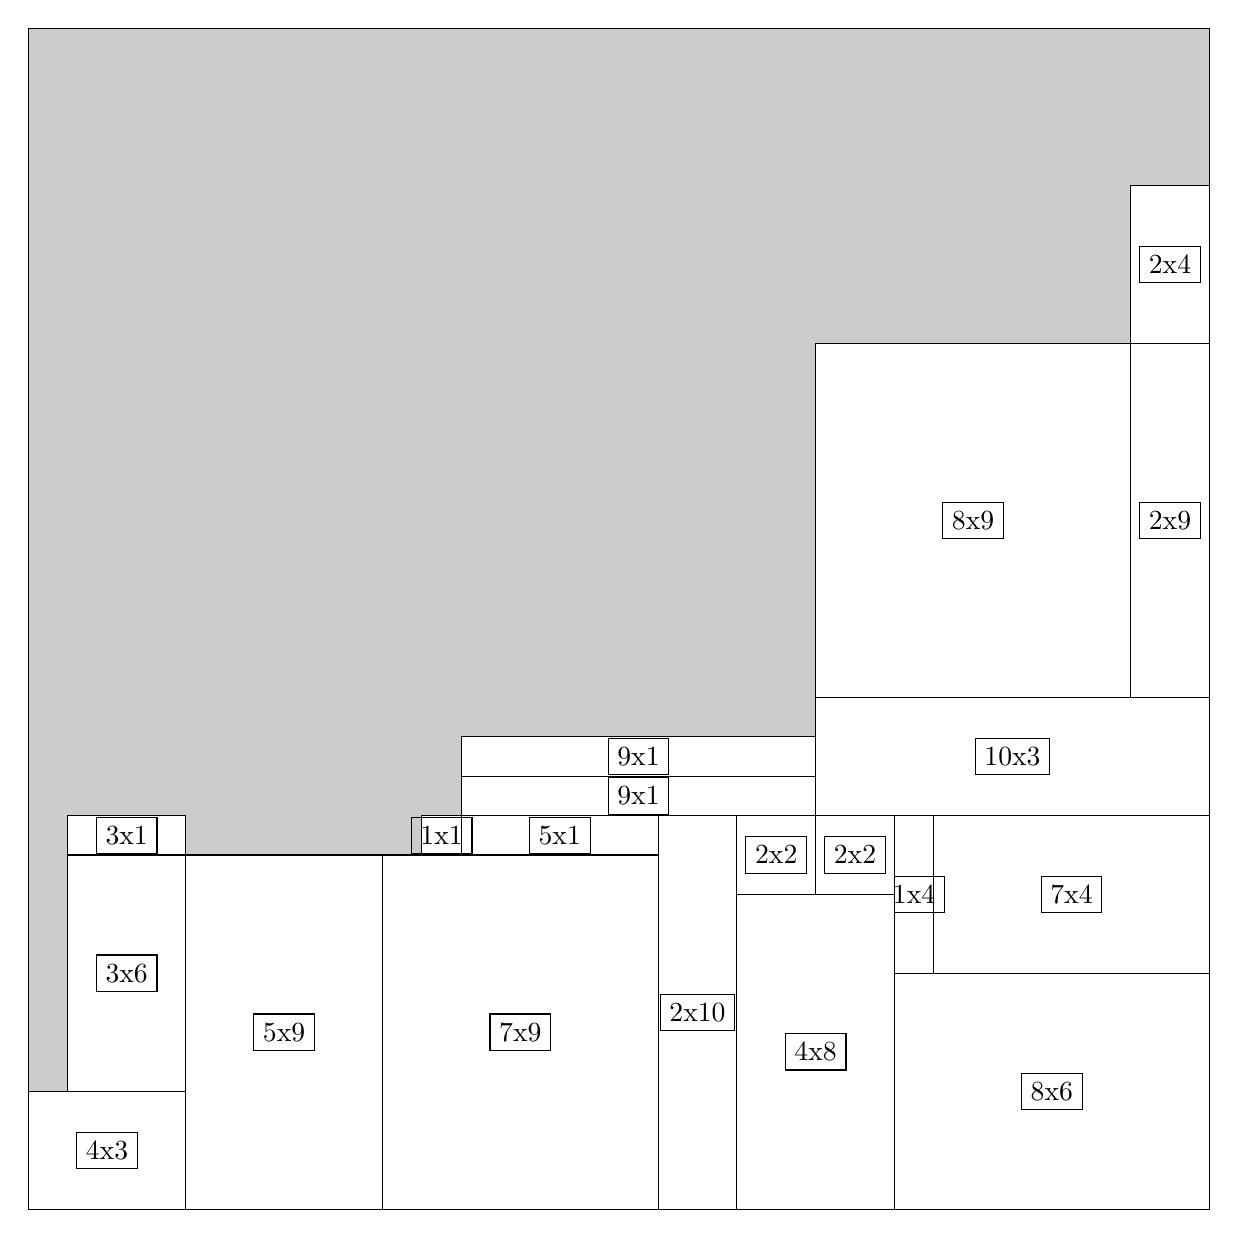
\begin{tikzpicture}[shorten >=1pt,scale=1.0,every node/.style={scale=1.0},->]
\tikzstyle{vertex}=[circle,fill=black!25,minimum size=14pt,inner sep=0pt]
\filldraw[fill=gray!40!white, draw=black] (0,0) rectangle (15.0,15.0);
\foreach \name/\x/\y/\w/\h in {8x6/11.0/0.0/4.0/3.0,7x4/11.5/3.0/3.5/2.0,1x4/11.0/3.0/0.5/2.0,4x8/9.0/0.0/2.0/4.0,2x2/10.0/4.0/1.0/1.0,2x2/9.0/4.0/1.0/1.0,2x10/8.0/0.0/1.0/5.0,7x9/4.5/0.0/3.5/4.5,5x1/5.5/4.5/2.5/0.5,1x1/5.0/4.5/0.5/0.5,5x9/2.0/0.0/2.5/4.5,4x3/0.0/0.0/2.0/1.5,3x6/0.5/1.5/1.5/3.0,3x1/0.5/4.5/1.5/0.5,10x3/10.0/5.0/5.0/1.5,9x1/5.5/5.0/4.5/0.5,9x1/5.5/5.5/4.5/0.5,2x9/14.0/6.5/1.0/4.5,2x4/14.0/11.0/1.0/2.0,8x9/10.0/6.5/4.0/4.5}
\filldraw[fill=white!40!white, draw=black] (\x,\y) rectangle node[draw] (\name) {\name} ++(\w,\h);
\end{tikzpicture}


w =8 , h =6 , x =22 , y =0 , v =48
\par
w =7 , h =4 , x =23 , y =6 , v =28
\par
w =1 , h =4 , x =22 , y =6 , v =4
\par
w =4 , h =8 , x =18 , y =0 , v =32
\par
w =2 , h =2 , x =20 , y =8 , v =4
\par
w =2 , h =2 , x =18 , y =8 , v =4
\par
w =2 , h =10 , x =16 , y =0 , v =20
\par
w =7 , h =9 , x =9 , y =0 , v =63
\par
w =5 , h =1 , x =11 , y =9 , v =5
\par
w =1 , h =1 , x =10 , y =9 , v =1
\par
w =5 , h =9 , x =4 , y =0 , v =45
\par
w =4 , h =3 , x =0 , y =0 , v =12
\par
w =3 , h =6 , x =1 , y =3 , v =18
\par
w =3 , h =1 , x =1 , y =9 , v =3
\par
w =10 , h =3 , x =20 , y =10 , v =30
\par
w =9 , h =1 , x =11 , y =10 , v =9
\par
w =9 , h =1 , x =11 , y =11 , v =9
\par
w =2 , h =9 , x =28 , y =13 , v =18
\par
w =2 , h =4 , x =28 , y =22 , v =8
\par
w =8 , h =9 , x =20 , y =13 , v =72
\par
\newpage


\end{document}